\chapter{Десорбция дейтерия из вольфрама при лазерном нагреве}\label{ch:ch4}

В настоящее время активно ведется разработка методов дистанционного контроля содержания изотопов водорода, которые основаны на взаимодействии лазерного излучения с поверхностью ОПЭ. Одним из таких перспективных подходов является лазерно-индуцированная десорбция (ЛИД). Этот метод включает в себя нагрев части поверхности с помощью лазерного импульса с последующим анализов вышедших частиц. Процедура ЛИД была успешно протестирована на нескольких токамаках, и сейчас ведется работа над созданием соответствующего комплекса для проекта ИТЭР~\cite{Zlobinski2024}. Ключевой задачей в этом процессе является определение оптимальных режимов работы, а также оценка возможных источников погрешности в измерениях.

Для применения в ЛИД рассматриваются лазерные системы с длительностью импульса вплоть до нескольких миллисекунд. Импульсный нагрев с большей длительностью позволяет проводить анализ содержания изотопов водорода на большей глубине~\cite{Yu2019, Zlobinski2020}, когда короткие импульсы (порядка наносекунд) позволяют исследовать тонкий поверхностный слой~\cite{Gasparyan2021}. Примечательно, что длительность на уровне миллисекунд сопоставима с длительностью импульсных нагрузок во время ELM-событий. С математической точки зрения, обе задачи весьма похожи, что позволяет проводить анализ в рамках одного подхода.

Беря во внимание недавнее решение Международный организации ИТЭР о переходе к полностью вольфрамовой облицовке, актуальным вопросом является исследование ЛИД изотопов водорода из вольфрамовых слоев. Также необходимо напомнить, что в услоиях токамака основным каналом накопления изотопов водорода является соосаждение. Этот механизм приводит к образованию пленок на поверхности ОПЭ, теплофизические свойства которых могут отличаться от случая материалов с идеальной структурой. В данной главе на основе численного моделирования проводится анализ закономерностей выхода дейтерия из вольфрама при импульсном лазерном нагреве. Рассматривается влияние различных эффектов, связанных как с процессами на поверхности, так и с параметрами материала. Как и в прошлой главе, сначала перед представлением основных результатов моделирования в данной главе проводится оценка применимости используемого подхода основе сравнения с экспериментальными данными, полученными в экспериментах на КСПУ-Т~\cite{Poskakalov2020}. \fixme{Все исходные коды в программном пакете FESTIM и результаты проведенных расчетов также распространяются свободно. ССЫЛКА НА ГИТ И ЗЕНОДО}

\section{Моделирование эксперимента по ЛИД дейтерия и соосажденных пленок вольфрама}\label{sec:ch4/sec1}

\subsection{Детали эксперимента}\label{subsec:ch4/sec1/subsec1}

Эксперименты по ЛИД проводились на базе физико-технического института им. А. Ф. Иоффе. В них использовались пленки вольфрама, соосажденные с дейтерием. Пленки были нанесены на медные подложки ($20 \times 20 \times \SI{3}{\milli\metre}$) методом импульсного лазерного осаждения в атмосфере дейтерия (давление \SI{30}{\pascal}) с плазменным ассистированием при частоте \SI{13.56}{\mega\hertz}. Для осаждения плёнок вольфрама использовался твердотельный лазер Nd:YAG с длиной волны \SI{1064}{\nano\meter}, энергией в импульсе \SI{1.3}{\joule}, длительностью импульса \SI{12}{\nano\second} и частотой следования импульсов \SI{10}{\hertz}. Лазерное излучение фокусировалось на вольфрамовой мишени для обеспечения плотности энергии $\approx\SI{25}{\joule\per\centi\meter\squared}$. Осаждение проводилось в течение 15 минут при водяном (\SI{18}{\degreeCelsius}) охлаждении держателя подложки. Измеренная толщина осажденных пленок составила $\approx\SI{1}{\micro\metre}$.

Полученные образцы укладывались на медное основание ($100 \times 80 \times \SI{3}{\milli\metre}$). Для обеспечения лучшего теплоотвода во время ЛИД между медным основанием и образцами устанавливались индиевые прокладки. Композитная мишень фиксировалась медной рамкой с окошками, как показано на рисунке~\cref{fig:ch4/LID_target}. Образцы облучались лазерными импульсами с длительностью \SI{220}{\micro\second} и \SI{1}{\milli\second} (оптоволоконная лазерная система, IPG YLR-2000, \SI{1070}{\nano\metre}). Для ясности далее в работе первый случай будет относиться к микросекундному нагреву, а второй "--- к миллисекундному. Полная энергия лазерных импульсов варьировалась в диапазоне от \SI{0.12}{\joule} до \SI{0.35}{\joule} и от \SI{0.25}{\joule} до \SI{1.00}{\joule} для микросекундной (\( \SI{220}{\micro\second} \)) и миллисекундой (\(\SI{1}{\milli\second}\)) длительности импульса соответственно. Анализ образцов после проведения ЛИД не показал явных изменений поверхности.

\begin{figure}[ht]
    \centerfloat{
        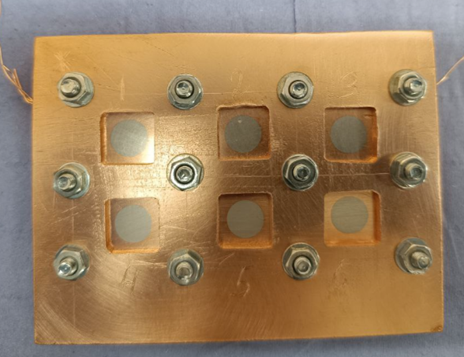
\includegraphics[scale=0.7]{LID_target.png}
    }
    \caption{Вид образцов с пленками вольфрама, расположенных на медном основании. Серые области "--- вольфрам-дейтериевые пленки}\label{fig:ch4/LID_target}
\end{figure}

Пространственный профиль плотности энергии измерялся лазерным анализатором SP620U OPHIR-SPIRICON. Полученный профиль соответствовал распределению Гаусса с усредненным значением полной ширины на уровне $1/e^2$ равным \(\mathrm{FW}=\SI{1}{\milli\metre}\) (удвоенное стандартное отклонение соответственно \SI{0.5}{\milli\meter}). Временные профили лазерного импульса измерялись кремниевым фотодиодом ФДУК-200 в фотогальваническом режиме. Временной профиль имели прямоугольную форму с характерной длительностью нарастания/затухания импульса равной \( \approx \SI{10}{\micro\second} \). Экспериментальный стенд для исследования ЛИД (см. рисунок~\ref{fig:ch4/LID_scheme}) включал в себя оптическую схему на основе двухлинзовой фокусирующей системы Галилея, систему перемещения лазерного луча по поверхности и вакуумный объём ($\approx\SI{70}{\liter}$). Вакуумный объём откачивался турбомолекулярным насосом (Turbovac 90i, Leybold) до базового уровня давления \SI{8e-5}{\pascal}.

\begin{figure}[ht]
    \centerfloat{
        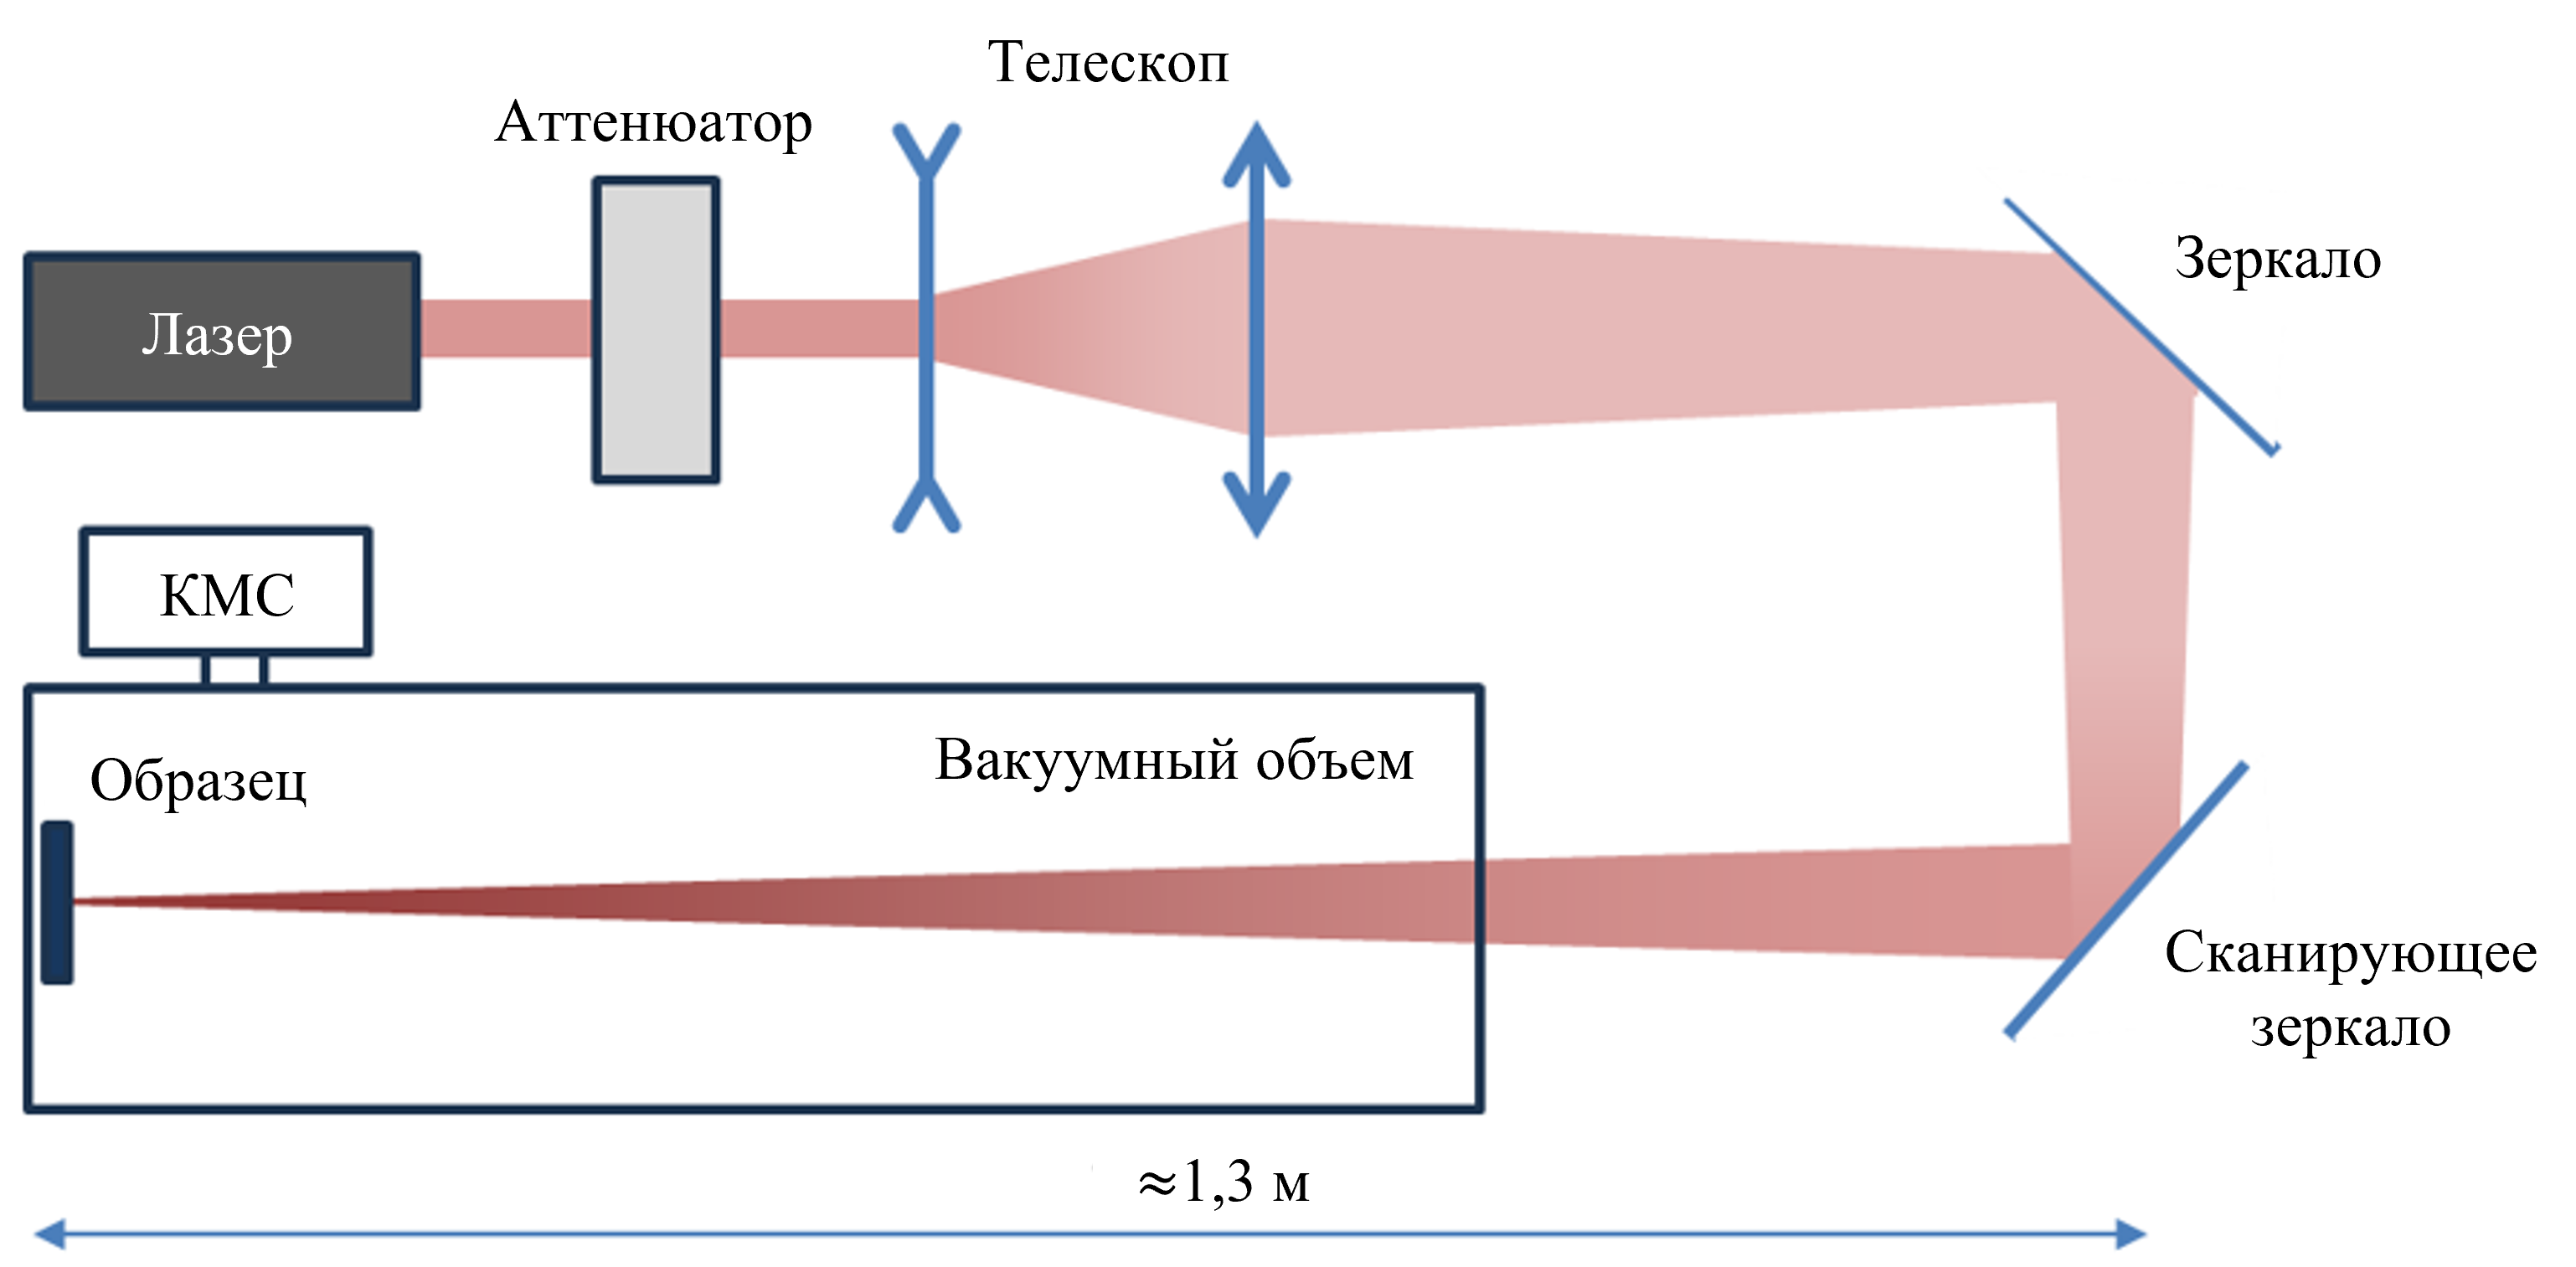
\includegraphics[scale=0.65]{LID_optic_scheme_ru.png}
    }
    \caption{Схема установки для проведения измерений ЛИД~\cite{Medvedev2024}}\label{fig:ch4/LID_scheme}
\end{figure}

Серия измерений при каждой длительности лазерного пучка проводились на отдельном образце. Участки поверхности образцов облучались серией импульсов с частотой \SI{0.1}{\hertz}. Регистрация сигналов 2; 3 и 4 масс проводилась с помощью КМС (Extorr XT300M). Масс-спектрометр калибровался по постоянному потоку дейтериевой течи с уровнем потока \SI{e-6}{\metre\cubed\pascal\per\second}. В ходе экспериментов изменения в сигналах 3 и 4 масс были ярко выражены, когда сигнал 2-ой массы не отличался от фонового. После серии импульсов энергия лазерного пучка и облучаемая область поверхности менялись. Смещение лазерного пятна происходило на такое расстояние, чтобы избежать влияния предыдущих импульсов на результаты измерений последующих. Для упрощения сравнения результатов численного моделирования с экспериментом из каждой серии импульсов при различных энергиях пучка использовались только первые выстрелы. Откалиброванный сигнал от первого выстрела интегрировался по времени для определения полного числа десорбированных атомов дейтерия. Статистическая погрешность измерений была оценена на уровне 20\%. Температура поверхности образцов в ходе экспериментов не измерялась ввиду ограничений экспериментального стенда.

Получение дополнительной информации о параметрах центров захвата в осажденных пленках осуществлялось методом ТДС. Были исследованы аналогичные образца с соосажденными пленками, толщиной \SI{0.5}{\micro\metre}. Измерения проводились на сверхвысоковакуумном стенде \thesisOrganizationShort \ (кафедра №21)~\cite{Rusinov2009} с постоянной скоростью нагрева \SI{0.5}{\kelvin\per\second}. Сигналы десорбированных молекул регистрировались КМС (HIDEN), работающим с использованием метода пороговой ионизации. Калибровка масс-спектрометра проводилась в соответствии с процедурой, описанной в работе~\cite{Rusinov2009}.

\subsection{Расчетная модель}\label{subsec:ch4/sec1/subsec3}

С целью воспроизведения результатов экспериментальных измерений ЛИД дейтерия из вольфрама была рассмотрена упрощенная геометрическая модель в цилиндрических координатах с аксиальной симметрией (см. рисунок~\cref{fig:ch4/LID_geom}), состоящая из двух материалов: вольфрамовой пленки (\SI{1}{\micro\meter}) и медной подложки (\SI{6}{\milli\meter}). Радиус расчетной области был выбран равным \SI{2}{\milli\meter}. На таком радиусе интенсивность лазерного импульса существенно затухает (в \( 1/e^{32} \) раз). Характерный масштаб распространения тепла за время лазерного воздействия с миллисекундной длительностью составляет \( L_\mathrm{heat}=\sqrt{\kappa \tau_\mathrm{ms}/C_p \rho} \approx \SI{0.2}{\milli\meter} \), что также не превышает величины радиального размера геометрической модели. Толщина геометрии была выбрана в соответствии с параметрами образцов.

\begin{figure}[ht]
    \centerfloat{
        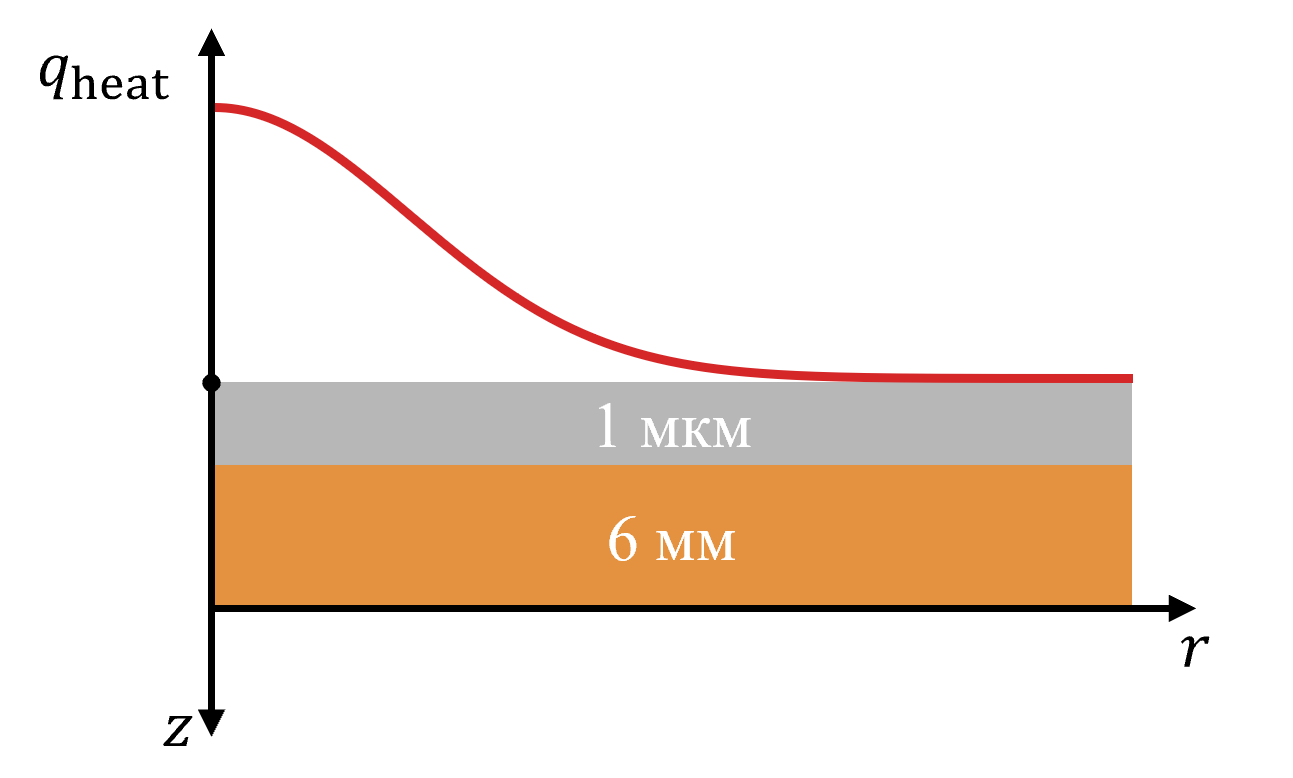
\includegraphics[scale=1]{LID_geom.png}
    }
    \caption{Схематическое представление двумерной геометрической модели, использованной при расчетах ЛИД. Радиус модели \SI{2}{\milli\meter}; \cruleme[customgrey]{0.5cm}{0.5cm}~---~W; \cruleme[customorange]{0.5cm}{0.5cm} "--- Cu}\label{fig:ch4/LID_geom}
\end{figure}

Было рассмотрено однородное уравнение теплопроводности в приближении идеального теплового контакта между пленкой и подложкой:
\begin{align}
    C_p \rho \frac{\partial T}{\partial t} = \frac{1}{r}\frac{\partial}{\partial r}\left( \kappa r \frac{\partial T}{\partial r} \right) + \frac{\partial }{\partial z}\left( \kappa \frac{\partial T}{\partial z} \right).
\end{align}
Температурная зависимость теплофизических свойств вольфрама и меди определялась уравнениями~\cref{eq:app/W_props,eq:app/Cu_props}. Нагрев за счет лазерного воздействия моделировался в качестве плотности мощности на границе:
\begin{equation}
    -\kappa \left. \frac{\partial T}{\partial z} \right\vert_{z=0} = q(r, t),
\end{equation}
Данное приближение справедливо, когда глубина проникновения лазерного излучения в твердое тело намного меньше характерного пространственного масштаба переноса тепла. Для вольфрама глубина проникновения излучения в ближнем инфракрасном диапазоне составляет величину \( \sim \SI{10}{\nano\meter} \)~\cite{Ordal1988}. Характерный масштаб переноса тепла при микросекундном нагреве можно оценить на уровне \( \sim \SI{0.1}{\milli\meter} \), что подтверждает справедливость приближения. Потерями мощности на излучение пренебрегается по сравнению с лазерным нагревом~\cite{Stepanenko2024}. Интенсивность лазерного импульса определялась на основе экспериментальных данных:
\begin{equation}
    q(r,t)=\frac{A E_\mathrm{laser}}{2\pi \sigma_{r}^2\tau_\mathrm{imp}} \exp \left( -\frac{r^2}{2 \sigma_r^2} \right) \eta \left( \tau_\mathrm{imp}-t \right),
\end{equation}
где \(A \) "--- коэффициент поглощения лазерного излучения; $E_\mathrm{laser}$ "--- полная энергия лазерного импульса, \si{\joule}; $\sigma_r=\mathrm{FW}/4=\SI{0.25}{\milli\meter}$ "--- стандартное отклонение пространственного распределения; \( \tau_\mathrm{imp} \) "--- длительность лазерного импульса, с; \(\eta(x)\) "--- функция Хевисайда. Передний/задний фронт во временной зависимости интенсивности лазерного импульса не учитывались. На остальных границах температура была фиксирована и равна начальной \(T_0=\SI{300}{\kelvin}\). Коэффициент поглощения лазерного излучения зависит от длины волны, температуры и состояния поверхности. На длине волны \SI{1070}{\nano\meter} он варьируется от \num{0.35} до \num{0.4} в области температур до \( \approx \SI{900}{\kelvin} \)~\cite{Minissale2017}. В ходе экспериментов состояние поверхности и ее температура не контролировались, что не позволяет провести сравнение результатов расчета эволюции температуры материала для уточнения значения параметра. Учитывая метод нанесения пленок, можно предположить, что коэффициент поглощения будет больше, чем в случае чистого вольфрама. В последующей части раздела этот параметр расценивался как свободный.

Задача транспорта дейтерия рассматривалась только для области вольфрама в силу того, что возможное проникновения дейтерия в медь не могло существенно влиять на сигнал измерений в режиме однократного облучения поверхности. Эволюция концентрации подвижных атомов дейтерия определялась из:
\begin{align}
    \frac{\partial \cm}{\partial t} = -\frac{1}{r}\frac{\partial (r J_r )}{\partial r} - \frac{\partial J_z}{\partial z} - \sum\limits_i \frac{\partial \cti}{\partial t},
\end{align}
где компоненты диффузионного потока определяются соответствующими компонентами градиентов концентрации и температуры. Процессы захвата и освобождения из дефектов определялись уравнением~\cref{eq:ch2/trapped_conc}. Полагалось, что все центры захвата распределены равномерно в слое вольфрама, что обычно справедливо для соосажденных пленок~\cite{Krat2020_2}. Начальная концентрация подвижных атомов была равна нулю, когда все дефекты считались полностью заполненными. На облучаемой поверхности задавалась нулевая концентрация подвижных атомов (приближение мгновенной десорбции), когда на остальных границах "--- нулевой поток. Параметры, определяющие транспорт дейтерия и сопутствующие процессы, приведены в таблице~\cref{tab:W_props}. Расчеты проводились на неоднородной сетке, линейный размер элементов которой увеличивался от поверхности вольфрама (\SI{10}{\nano\meter}) до поверхности меди (\SI{0.1}{\milli\meter}). Модельное время составляло \SI{0.1}{\second}, чего было достаточно для окончания десорбции и охлаждения материалов до начальной температуры. Величина временного шага интегрирования во время действия тепловой нагрузки не превышала \num{2.5} и \SI{25}{\micro\second} для микросекундного и миллисекундного случаев.

Определение параметров центров захвата (количество, концентрация, барьер освобождения) проводилось путем анализа ТДС-спектра на основе методики~\cite{Delaporte-Mathurin2021}, описанной ранее в настоящей работе. Моделирование проводилось в одномерном приближении. Температура было однородна по образцу и менялась линейно со временем. Параметры моделирования, граничные и начальные условия аналогичны тем, что использовались в задаче ЛИД.

\subsection{Сравнение результатов моделирования и эксперимента}\label{subsec:ch4/sec1/subsec4}

Экспериментальный ТДС-спектр удалось воспроизвести в предположении наличия четырех типов центров захвата:
\begin{enumerate}[beginpenalty=10000]
    \item \( n_\mathrm{t,1}=\SI{2.89}{\text{ат.}\percent} \), \( E_\mathrm{dt,1}=\SI{1.108}{\electronvolt} \);
    \item \( n_\mathrm{t,2}=\SI{1.79}{\text{ат.}\percent} \), \( E_\mathrm{dt,2}=\SI{1.279}{\electronvolt} \);
    \item \( n_\mathrm{t,3}=\SI{1.97}{\text{ат.}\percent} \), \( E_\mathrm{dt,3}=\SI{1.536}{\electronvolt} \);
    \item \( n_\mathrm{t,4}=\SI{0.60}{\text{ат.}\percent} \), \( E_\mathrm{dt,4}=\SI{1.818}{\electronvolt} \).
\end{enumerate}
На рисунке~\cref{fig:ch4/LID_TDS} приведены экспериментальный и модельный ТДС-спектры дейтерия из соосажденных пленок вольфрама. Также явно показан вклад от каждого типа дефекта в поток десорбированных частиц.

\begin{figure}[ht]
    \centerfloat{
        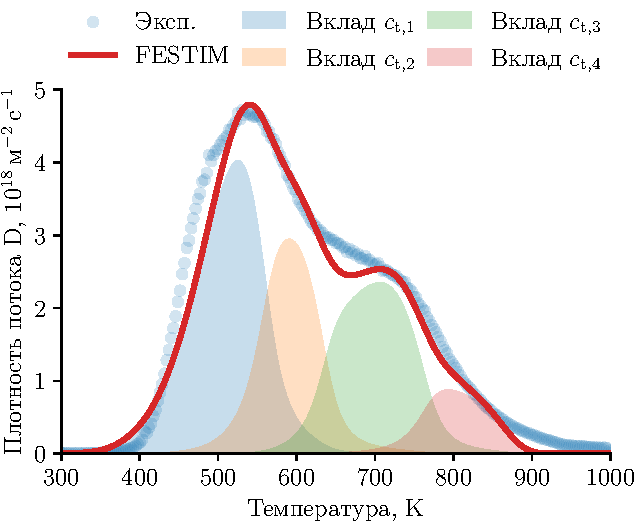
\includegraphics[scale=1]{LID_TDS.pdf}
    }
    \caption{Сравнение ТДС-спектров дейтерия из соосажденных пленок вольфрама, рассчитанного в коде FESTIM и измеренных в эксперименте}\label{fig:ch4/LID_TDS}
\end{figure}

Оцененное содержание дейтерия в пленках составляет более 7 ат.\%. Параметры центров захвата дейтерия согласуются с данными, приведенными в литературе для слоев соосаждения вольфрама~\cite{Krat2018}. Барьер выхода дейтерия \SIrange{1.0}{1.5}{\electronvolt} может соответствовать вакансиям в решетке вольфрама, занятыми одним (\(\approx\SI{1.5}{\electronvolt}\)) или несколькими атомами дейтерия (\(<\SI{1.5}{\electronvolt}\)), когда центр захвата с наибольшим барьеров выхода (тип 4) может соответствовать выходу дейтерия из вакансионного кластера~\cite{Ogorodnikova2015}. Полученные параметры дефектов были далее использованы для моделирования ЛИД.

\fixme{На рисунке показаны распределения поля температуры при достижении максимального значения для двух длительностей лазерного импульса. Максимальная температура поверхности при длительности импульса в 1 мс составила 1000 К, когда при длительности в 220 мкс – 850 К. Из распределений профилей температуры следует, что во время лазерного воздействия прогревается область с радиусом ≈1 мм. На нижней паре графиков на рисунке 6 распределения содержания дейтерия после облучения, когда выход дейтерия прекращается. Из сравнения результатов для двух длительностей следует, что при примерно одинаковой пиковой температуре поверхности эффективность ЛИД выше при использовании более длительного импульса. Однако в обоих случаях радиус анализируемой области составляет ≈0,5 мм, что соответствует полуширине пространственного профиля энергии лазерного импульса.}

Была проведена серия моделирований по ЛИД дейтерия из вольфрамовых пленок при различных длительностях и энергиях лазерного импульса. Для каждого случая было определено полное число десорбированных атомов дейтерия за импульс. Сравнение результатов моделирования и экспериментальных измерений представлено на рисунке~\cref{fig:ch4/LID_Comparison}. Результаты, полученные путем моделирования, качественно описывают экспериментально измеренные зависимости. Для обеих длительностей импульсов наблюдается рост числа вышедших частиц с увеличением энергии, вложенной в лазерный импульс. Число десорбированного дейтерия также оказывается выше при предельной тепловой нагрузке в случае использования миллисекундного ЛИД.

\begin{figure}[ht]
    \centerfloat{
        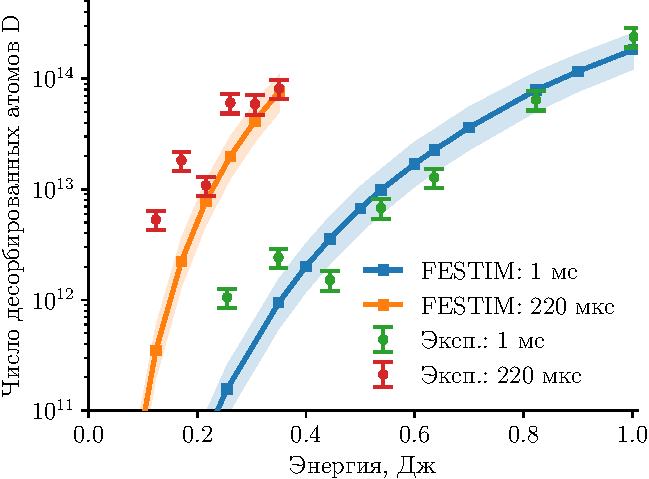
\includegraphics[scale=1]{LID_Comparison.pdf}
    }
    \caption{Сравнение расчетных и экспериментальных зависимостей числа десорбированных частиц от энергии лазерного импульса. Сплошные линии соответствуют коэффициенту поглощения излучения \( A=0.55 \), закрашенные области~"---~\( A = 0.5-0.6 \)}\label{fig:ch4/LID_Comparison}
\end{figure}

Однако между результатами численного моделирования и экспериментальных измерений наблюдается количественное расхождение, наиболее явно наблюдающееся при длительности нагрева в 220 мкс. Более точное измерение параметров нагрева и/или температуры пленки во время ЛИД (например, температуры ее поверхности) позволит уточнить решение задачи о переносе тепла и минимизировать влияние неизвестных параметров.

\section{Анализ состава потока десорбированных частиц}\label{sec:ch4/sec2}

Анализ ТДС-экспериментов обычно основывается на предположении о молекулярной рекомбинации на поверхности. Некоторые эмпирические результаты предполагают возможность прямой десорбции атомов. Ранне отмечалось, что капиллярные источники атомарного водорода основаны на термической диссоциации инжектированных молекул на горячих стенках. Степень атомизации в таких установках может превышать 90\% при температурах выше \SI{2400}{\kelvin} и плотностью потока напускаемого газа \SIrange{e20}{e22}{\per\meter\squared\per\second}~\cite{Tschersich2000,Tschersich2008}. Во время ЛИД могут быть достигнуты соизмеримые температуры поверхности, однако плотность потока частиц, десорбированных после мощного лазерного облучения, может быть значительно больше, чем в ТДС, и варьируется в зависимости от длительности импульса. Плотность потока была оценена на уровне \SI{e27}{\per\meter\squared\per\second} при использовании коротких импульсов с наносекундной длительностью~\cite{Gasparyan2021}, что предполагает большую вероятность выхода молекул с поверхности. Возможный выход атомов можно ожидать при более длительных импульсов, когда соответствующая плотность потока оказывается на несколько порядков меньше~\cite{Yu2019}.

Возникновение фракции атомов в потоке десорбированных частиц может влиять на точность измерений. Количественный анализ числа вышедших атомов в ЛИДС основан на измерении фотонного потока, испущенного при ионизации в пристеночной плазме. Коэффициенты пропорциональности между потоками определяются типом частиц и характерными механизмами их ионизации. В условиях токамака TEXTOR было показано увеличение (снижение) вклада от десорбированных атомов (молекул) в регистрируемый фотонный поток в зависимости от температуры графитового лимитера~\cite{Brezinsek2005}. В качестве основных механизмов указываются ионизация атомов электронным ударом и диссоциация молекул после ионизации электронным ударом, что в обоих случаях приводит к эмиссии одного фотона и требует учета при интерпретации спектроскопических измерений. Следует подчеркнуть, что пример приведен для графитовой поверхности, процессы десорбция изотопов водорода с которой отличаются от случая металлических поверхностей. Однако процедура спектроскопических измерений остается прежней. Выход атомов с поверхности также может вносить погрешность в результаты измерений, полученных с помощью КМС, так как вероятность достижения атомами измерительного прибора может быть меньше, чем в случае молекулы, из-за большего коэффициента прилипания к поверхности. Таким образом, информация о величине атомарной фракции в потоке десорбированных частиц во время ЛИД может иметь значение для проведения точной обработки результатов измерений.

\subsection{Постановка задачи}\label{subsec:ch4/seс2/subsec1}
Оценка атомарной фракции в потоке десорбированных частиц проводилась на основе численных модели ЛИД дейтерия из вольфрама в одномерном приближении~\cite{Kulagin2023}. Данное приближение не повлияет на основные выводы раздела и может в разумных пределах воспроизводить результаты двумерных расчетов, когда радиус лазерного пятна превышает характерные масштабы переноса тепла и транспорта дейтерия~\cite{Stepanenko2024}. Задача о переносе тепла определялась аналогично прошлому разделу:
\begin{subequations}
    \begin{align}
        C_p \rho \frac{\partial T}{\partial t}                         & = \frac{\partial}{\partial x}\left( \kappa \frac{\partial T}{\partial x} \right), \\
        -\kappa \left. \frac{\partial T}{\partial x} \right\vert_{x=0} & = \frac{E_0}{\tau_\mathrm{imp}} w(t),
    \end{align}
\end{subequations}
где \( E_0 \) "--- плотность энергии лазерного импульса, \si{\joule\per\meter\squared}; \( \tau_\mathrm{imp} \) "--- длительность лазерного импульса, с; \(w(t) \) "--- временной профиль импульса. На обратной стороне температура была фиксирована и равна начальной \(T_0=\SI{300}{\kelvin}\). Теплофизические свойства вольфрама задавались на основе выражений~\cref{eq:app/W_props}.

Чтобы исследовать влияние длительности нагрева, рассматривалось три случая, соответствущих экспериментальным работам~\cite{Zlobinski2019,Zlobinski2020,Gasparyan2021}:
\begin{itemize}
    \item наносекундный нагрев с гауссовым временным профилем при положении максимума \( t_0 = \SI{40}{\nano\second} \) и шириной \(\tau_\mathrm{ns}=\SI{25}{\nano\second} \);
    \item микросекундный нагрев с прямоугольным временным профилем, определяемым кусочно-гладкой функцией~\cref{eq:ch3/pulse_form} при \(\tau_\mathrm{le}=\tau_\mathrm{te}=\SI{0.5}{\micro\second}\), \(t_1=\SI{0.5}{\micro\second}\), \( t_2=\SI{2.5}{\micro\second}\), \( \Delta=\num{0} \);
    \item миллисекундный нагрев с трапециевидным временным профилем, определяемым кусочно-гладкой функцией~\cref{eq:ch3/pulse_form} при \(\tau_\mathrm{le}=\tau_\mathrm{te}=\SI{0.05}{\milli\second}\), \(t_1=\SI{0.25}{\milli\second}\), \( t_2=\SI{4.95}{\milli\second}\), \( \Delta=\num{-0.3} \).
\end{itemize}
Временные профили импульсов представлены на рисунке~\cref{fig:ch4/laser_time_profiles}.
\begin{figure}[ht]
    \centerfloat{
        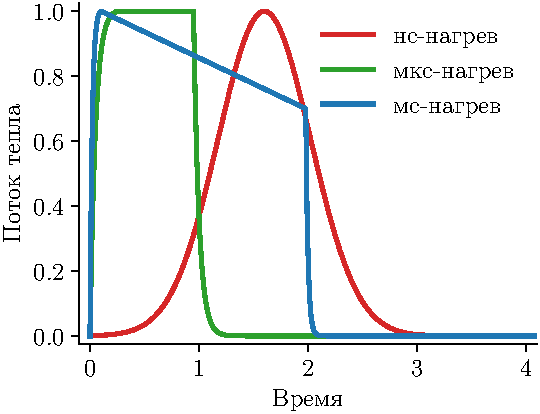
\includegraphics[scale=1]{laser_time_profiles.pdf}
    }
    \caption{Временные зависимости потоков тепла, использовании при моделировании лазерного нагрева различной длительности. Потоки нормированы на максимальное значение.  Длительности импульсов нормированы на \SI{25}{\nano\second}, \SI{10}{\micro\second} и \SI{2.5}{\micro\second} для наносекундного, микросекундного и миллисекундного случаев соответственно. }\label{fig:ch4/laser_time_profiles}
\end{figure}
Максимальное значение плотности энергии выбиралась таким образом, чтобы максимальная температура в ходе нагрева не достигала точки плавления. Для нано-, микро-, и миллисекундной длительности она составила величину \SI{10,2}{\kilo\joule\per\meter\squared}; \SI{160.1}{\kilo\joule\per\meter\squared} и \SI{3,8}{\mega\joule\per\meter\squared} соответственно.

В задаче транспорта учитывалось взаимодействие только с одним типом центров захвата (аналогично постановке задачи~\cref{eq:ch3/QSPA_diffusion}), равномерно распределенных в слое толщиной \SI{10}{\micro\meter} с концентрацией \SI{1}{\text{ат.}\percent} и барьеров выхода равным \SI{1.5}{\electronvolt}. Данный набор параметров можно отнести к захвату одного атома дейтерия в моновакансиях вольфрама~\cite{Krat2018}. Для анализа состава потока вышедших частиц на левой границе расчетной области рассматривалась модель, учитывающая кинетику процессов на поверхности. Ранее были предложены модели, учитывающие десорбцию молекул с участием как адсорбированных, так и приповерхностных атомов. Обобщение этих механизмов десорбции приведено в работе~\cite{Pisarev1997}. Полагаясь на более раний анализ, в настоящей работе рассматривается три процесса, приводящих к десорбции молекул. Все переходы качественно показаны на рисунке~\cref{fig:ch4/pot_diag_surf}. В явном виде плотность потока частиц в каждом из процессов определяется как:

\begin{subequations}
    \begin{align}
        J_\mathrm{m}^{\mathrm{s}}  & = 2\frac{\csurf^2}{n_\mathrm{s}} \nu_0 \exp \left( -2\frac{E_\mathrm{c}-Q_c(\theta)}{\kBT} \right),                                \\
        J_\mathrm{m}^{\mathrm{sb}} & = \csurf \frac{\cm}{n_\mathrm{IS}} \nu_0 \exp \left( -\frac{(E_\mathrm{c}-Q_c(\theta))+(E_\mathrm{s}-Q_\mathrm{s})}{\kBT} \right), \\
        J_\mathrm{m}^{\mathrm{b}}  & = 2 \frac{\cm^2}{n_\mathrm{IS}} \lambda_\mathrm{abs} \nu_0 \exp \left( -2\frac{E_\mathrm{s}-Q_\mathrm{s}}{\kBT} \right),
    \end{align}
\end{subequations}
где \( J_\mathrm{m}^{\mathrm{s}} \) "--- поток атомов в составе молекул, формируемый двумя адсорбированными атомами; \( J_\mathrm{m}^{\mathrm{sb}} \) "--- поток атомов в составе молекул, формируемый адсорбированным атомом и растворенным атомом вблизи поверхности; \( J_\mathrm{m}^{\mathrm{b}} \) "--- поток атомов в составе молекул, формируемый двумя растворенными атомами вблизи поверхности. 

Полагается, что в последних двух переходах растворенные атомы рекомбинируют между собой или с адсорбированным атомом и покидают материал, минуя хемосорбированное состояние. Важно подчеркнуть, что данное представление не является точным, так как выражения для констант скоростей процессов, по большей части, дают качественную оценку и построены исходя из размерности величин. Более обоснованное определение возможно, например, на основе DFT-анализа и потребует оценки соответствующих величин при различных конфигурациях атомов как на поверхности, так и в приповерхностном слое, что существенно усложняет задачу.

\begin{figure}[ht]
    \centerfloat{
        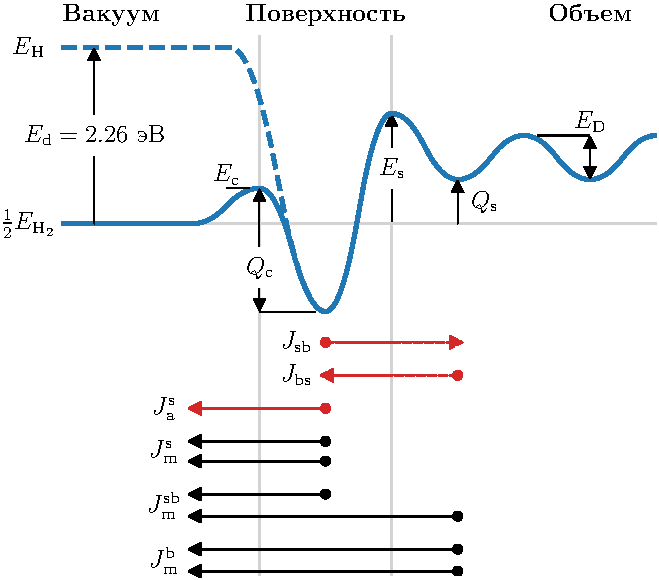
\includegraphics[scale=1]{potential_diagram_surface.pdf}
    }
    \caption{Упрощенная диаграмма потенциальной энергии атома дейтерия вблизи поверхности. Стрелки под диаграммой показывают возможные переходы атомов, учитываемые в моделировании}\label{fig:ch4/pot_diag_surf}
\end{figure}

Для оценки доли атомов в потоке вышедших частиц во время ЛИД был также рассмотрена прямая десорбция атомов. Плотность потока атомов определяется аналогично предыдущим величинам:
\begin{equation}
    J_\mathrm{a}^{\mathrm{s}} = \csurf \nu_0 \exp \left( -\frac{E_\mathrm{d}-Q_c(\theta)}{\kBT} \right).
\end{equation}
Во всех выражениях учитывается зависимость теплоты хемосорбции от концентрации адсорбированных атомов аналогично уравнению~\cref{eq:ch2/Edes_coverage} со следующими параметрами: \( Q_\mathrm{0} = \SI{0.071}{\electronvolt} \); \( \Delta Q = \SI{0.647}{\electronvolt} \); \( \theta_0=1.000 \); \( \delta \theta = \num{0.050} \). Эволюция концентрация атомов на поверхности и вблизи (\( x=0 \)) нее определяется следующими дифференциальными выражениями:
\begin{subequations}
    \begin{align}
        \frac{d \csurf}{dt}                                  & = \Jbs - \Jsb - J_\mathrm{a}^{\mathrm{s}} - J_\mathrm{m}^{\mathrm{s}} - J_\mathrm{m}^{\mathrm{sb}},      \\
        \lambda_\mathrm{abs} \frac{\partial \cm}{\partial t} & = -J_x+ \Jsb - \Jbs - J_\mathrm{m}^{\mathrm{b}} - J_\mathrm{m}^{\mathrm{sb}},
    \end{align}
\end{subequations}
где \( J_x \) "--- компонента диффузионного потока вдоль оси \(x\). В начальный момент времени концентрация дейтерия в объеме и на поверхности была равна нулю. На правой границе также задавалась нулевая концентрация дейтерия.

Значения постоянных, явно не указанные в разделе, обобщены в таблице~\cref{tab:W_props}. Длина расчетной геометрии \( L \) подбирался таким образом, чтобы температура на правой границе не менялась в ходе моделирования. Она была равна \SI{100}{\micro\meter}; \SI{1}{\milli\meter} и \SI{20}{\milli\meter} для случаев наносекундного, микросекундного и миллисекундного нагрева. Расчеты проводились на неоднородной сетки, размер элементов которой вблизи левой границы не превышал \SI{10}{\nano\meter}. Во время действия теплой нагрузки временной шаг был не менее чем на два порядка меньше ее характерной длительности.

Искомой величиной в настоящем разделе является атомарная фракция в потоке десорбированного дейтерия, которая определяется как:
\begin{equation}
    f_\mathrm{a} = \dfrac{\int\limits_0^\infty J_\mathrm{a}^\mathrm{s} dt}{\int\limits_0^\infty J_\mathrm{des} dt},
\end{equation}
где $J_\mathrm{des}=J_\mathrm{a}^{\mathrm{s}} + J_\mathrm{m}^{\mathrm{s}} + 2 J_\mathrm{m}^{\mathrm{sb}} + J_\mathrm{a}^{\mathrm{b}}$ "--- плотность полного потока десорбированных атомов. 

\subsection{Приближение равновесия вблизи поверхности}


\begin{subequations}
    \begin{align}
        J_\mathrm{d}(\beta_0 - \beta) & = \beta (1-\theta) K_{bs} - \theta (1-\beta) K_{sb} + 2\beta^2 K_m^b + \theta\beta K_m^{sb}                   \\
        0                             & = \beta (1-\theta) K_{bs} - \theta (1-\beta) K_{sb} - 2\theta^2 K_m^s - \theta\beta K_m^{sb} - \theta K_a^s .
    \end{align}
\end{subequations}

\begin{equation}
    \beta = \theta \dfrac{2\theta K_m^s + K_a^s + K_sb}{K_bs - \theta (K_bs + K_m^sb - K_sb)}
\end{equation}

\begin{equation}
    J_\mathrm{d} = 2\beta^2 K_m^b + 2\theta\beta K_m^sb + 2\theta^2 K_m^s + \theta K_a^s
\end{equation}

\begin{subequations}
    \begin{align}
        \theta       & = \frac{K_a^s}{4 K_m^s} \left( \sqrt{1+\dfrac{8J_\mathrm{des}K_m^s}{J_0 (K_a^s)^2}} -1 \right)                        \\
        f_\mathrm{a} & = \frac{О_0 (K_a^s)^2}{4 J_\mathrm{des} K_m^s} \left( \sqrt{1+\dfrac{8J_\mathrm{des}K_m^s}{J_0 (K_a^s)^2}} -1 \right)
    \end{align}
\end{subequations}

\subsection{Результаты численного моделирования}\label{subsec:ch4/seс2/subsec3}

В настоящем исследовании эффективность LID определяется как доля атомов, десорбированных после одного теплового импульса (    ∕ 0). Количество десорбированных атомов сильно зависит от параметров лазерного импульса. В основном, импульсные нагрузки с более высокой плотностью мощности соответствуют более высоким температурам материала. Нагрев до более высоких температур и поддержание материала при таких температурах в течение более длительного времени делают высвобождение H более вероятным [47]. Было показано, что пиковая температура поверхности является важным параметром для характеристики шероховатости поверхности PFC, развивающейся после воздействия кратковременных тепловых нагрузок [58,59]. Таким же образом можно оценить эффективность ЛИД, измерив максимальную температуру образца, достигнутую при нагревании

\section{Анализ влияния параметров материала на выход дейтерия}\label{sec:ch4/seс3}
\subsection{Влияние теплопроводности материала}\label{subsec:ch4/seс3/subsec1}
\subsection{Влияние параметров центров захвата}\label{subsec:ch4/seс3/subsec2}
\subsection{Режимы десорбции во время лазерно-индуцированной десорбции}\label{sec:ch4/seс3/subsec3}

\begin{subequations}
    \begin{align}
        \nu_des & \sim \frac{\nu_a}{2} \left( 1 + \sqrt{1+\dfrac{4J_\mathrm{des}\nu_m}{s\nu_a^2}} \right) \\
        \nu_D \sim \frac{D_\mathrm{eff}}{\delta_D}
    \end{align}

\end{subequations}

\section{Выводы к Главе~\ref{ch:ch4}}

\clearpage
